% !TEX root = ../main.tex
% Chapter 4

\chapter{Proposed method}

\label{Chapter4} % For referencing the chapter elsewhere, use \ref{Chapter4}

\lhead{Chapter 4. \emph{Proposed method}} % This is for the header on each page - perhaps a shortened title

%----------------------------------------------------------------------------------------
\section{Outline}
\emph{Not intented for the reader.}
\begin{itemize}
  \item Based on the problem statement with current research as stated in Chapter \ref{Chapter3}
  \item Adjust method to needs
  \item Explain using graphs, pseudo-algorithms. Make clear distinction in origin of ideas and why to apply
\end{itemize}


% !TEX root = ../../main.tex
\section{Change Indication}\label{sec:method_change_indication}
*** TODO: change section title ***
*** TODO: ***
\emph{Follow methodology of ``A unifying framework for detecting outliers and change points from time series'' \cite{takeuchi2006unifying}.
It creates a two-stage process of first searching for outliers, and then using the ``outlier-score'' to find (sudden) change points, by a weighted average of a moving window.
That eventual score can be thresholded (as in the paper) or processed with something like CUSUM (proposal).
Looks like my proposed methods, in that is combines outliers and gives a score to change points.}

The proposed method of this thesis follows the unifying framework as introduced by Takeuchi and Yamanishi \cite{takeuchi2006unifying} and an similar implementation by Camci \cite{camci2010change} with \glspl{svm}.
The unifying framework combines the detection of outliers with change points and divides it in two stages.
The first stage determines the outliers in a time series by giving a score based on the deviation from a learned model, and thereby creates a new time series.
The second stage runs on that new created time series and calculates a average over a window of the outlier scores.
The problem of change detection is then reduced to outlier detection over that average-scored time series.
This method is named \gls{changeFinder} by the authors.
The implementation by Camci, which uses \glspl{svm} to detect changes is named \acrlong{svcpd}.

The problem statement and formal definition, following Tackeuchi and Yamanishi \cite{takeuchi2006unifying} and Camci \cite{camci2010change} is the following.
The algorithm needs to find \emph{sudden} changes in the time series data.
In other words, slowly changing properties in the data are not considered to be changes.
This is in line with the search of changes in activities, since we are only interested in different activities (which are represented by sudden changes) instead of changes within an activity.
Considered a time series $x_1 x_1 \dots$, which is drawn from a stochastic process $p$.
Each $x_t$ (t = 1, 2, \dots) is a $d$-dimensional real valued vector and $p$ a probability density function of the sequence $x_1 x_2 \dots$.
Assume $p$ can be decomposed in two different \gls{iid} stationary stochastic processes $p^1$ and $p^2$ and are one-dimensional Gaussian density functions.
For a time point $a$ data points for which $t < a$ are drawn from $p^1 = N(\mu_1, \sigma_1^2)$ and for $t \geq a$ from $p^2 = N(\mu_2, \sigma_a^2)$.
If $p^1$ and $p^2$ are different, then the time point $t = a$ is a \emph{change point}.
In \cite{takeuchi2006unifying} the similarity between the stochastic processes are expressed by the \gls{kliep} divergence $D(p^2||p^1)$.
The problem with this measure is that, as the authors conclude and Camci discusses, it is not able to detect a change by decrease in variance.

Whereas \gls{changeFinder} uses double probability estimation algorithm, our approach follows \gls{svcpd} by constructing a \gls{svm} over a sliding window.
The \gls{svcpd} algorithm uses the location of new data points in the feature space $\mathcal{F}$ with respect to the hypersphere and the hypersphere's radius $R$ to determine whether the new data point represents a change point.

*** TODO: What is my contribution compared to Camci? Distance of outliers to hypersphere? ***
% !TEX root = ../../main.tex
\section{Overview}\label{sec:method_overview}

\begin{figure}
  \centering
    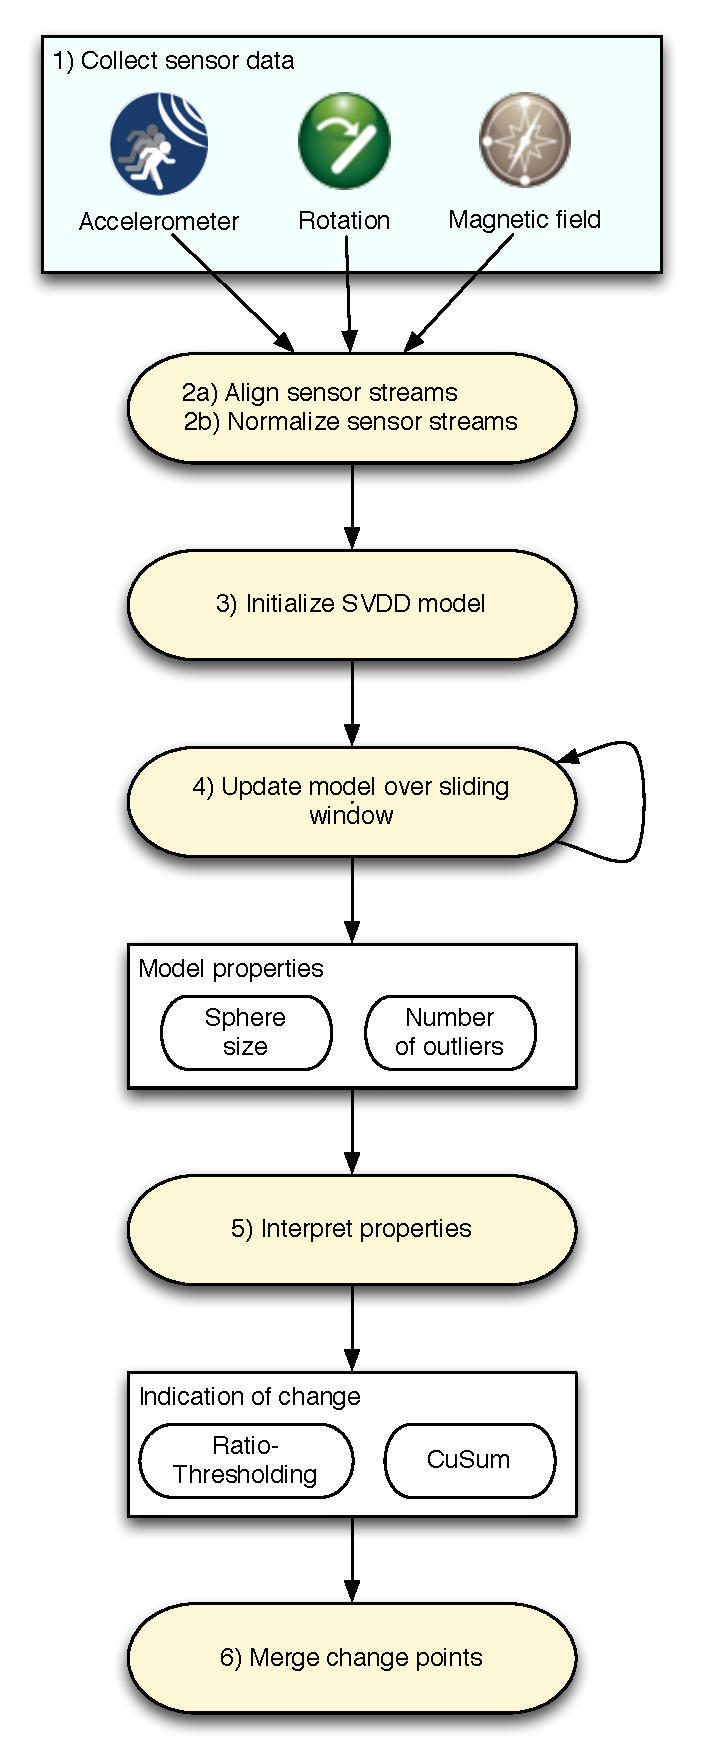
\includegraphics[width=\textwidth,height=\textheight,keepaspectratio]{./Figures/graphs/chapter4/method_setup.pdf}
  \caption[Method setup]{Schematic representation of the change detection method.}
  \label{fig:method_overview}
\end{figure}

This section gives a description of the method used for the experiments and change detection mechanism.
First described is the method to process the gathered sensor data.
A schematic overview is given in figure \ref{fig:method_overview} and shows the steps of the method.
A more detailed explanation of the ``Update model'' step follows.
This section is finalized with the experiments setup, annotation of data streams and quality measure.

\subsection{Change detection method}
As graphically represented in figure \ref{fig:method_overview}, the change detection method starts by processing the data from sensor, such as the accelerometer, magnetic orientation and rotation measures \footnote{Something about the origin of the streams; all from the same sensor or different sensors?}.

The first step is to process the raw streams of data originating from a multiple of sensors.
The two processes applied are alignment and normalization.
Due to noisy sampling, not all the timestamps in the data streams are sensed at the same timestamp.
Since the \gls{svdd} method requires all the data stream at every timestamp and can not handle missing data on one of the timestamps, all the unique timestamps are filtered out.
Whilst this results in an overall filtering effect, in practice between $1\%$ and $5\%$ of each data stream is disregarded.
The effect of this filtering is not significant and the data is not modified.

Due to the nature of the sensor signals, a normalization step is required in order to set the weight for all the data streams equal.
The range of the accelerometer signal typically spans $-20$ to $20$, the magnetic field from $-60$ to $60$ and the rotations range is from $-1$ to $1$.
This means that a relative small change in the accelerometer stream could have a much larger impact on the model than the same (absolute) change in the rotation stream, whilst the latter has a larger relative impact.
The normalization step ensures that all data is weighted equally and changes in the data are all proportional.

In step $3$ the \gls{svdd} model is initialized.
The first full window over the data stream is used to construct an initial model.
During the initialization the parameters for the \gls{svdd} are provided, begin the kernel type (radial), \gls{rbf} with $\sigma$ and the outlier-fraction $C$.

Step $4$ is executed for every step-size $s$ data points in the stream.
Every update the oldest $s$ data points are removed from and $s$ new data points are added to the \gls{svdd} model.
The model is (partially) reconstructed and new model properties, such as the radius of the hypersphere and the number of outliers, are the result of this step \footnote{Other measures are also possible, for instance the distance from all the outliers to the boundary of the hypersphere}.
*** MORE ON THE UPDATING STEP ***

This final step of this method, step $5$, is the interpretation of the model properties.
Many algorithms can be used for this process, all which take a one-dimensional time series as input and determine where change has occured.
In our setup we used the \gls{rt} and \gls{cusum} methods, to show the modularity of this step.

\subsection{Model updating}

\subsection{Experiments}
For the experiments we used a HTC Sensation XE smartphone as recording device.
The activities were recorded using a free Android application \cite{sensorlogger}.
This application was chosen for its convenient data format of the sensor recording and its regularity of the sampling interval.
Table \ref{tab:recorded_metrics} lists the recorded metrics.
For our expiments we used the data for the accelerometer, magnatief field and rotation.

\begin{center}\begin{table}
  \begin{tabulary}{\textwidth}{|l|L|c|c|}
    \hline
    Metric & Description & Units of measure & Typical range \\
    \hline \hline
    Accelerometer & Acceleration force along each axis. & $m/s^2$ & $-20$ -- $20$ \\
    \hline
    Gravity & Force of gravity along each axi.s & $m/s^2$ & $-10$ -- $10$\\
    \hline
    Gyroscope & & $rad/s$ & $-15$ -- $15$\\
    \hline
    Light & Light sensitive sensor at the front of the phone. & & $0$ -- $10000$ \\
    \hline
    Linear acceleration & & $m/s^2$ & $-20$ -- $20$ \\
    \hline
    Magnetic field & Geomagnetic field strength along each axis. & $\mu T$ & $-60$ -- $60$ \\
    \hline
    Orientation & & & $-100$ -- $360$ \\
    \hline
    Rotation & & & $-1$ -- $1$\\
    \hline
  \end{tabulary}
  \caption{Measured metrics. The set of axis is always the triple (x, y, z) direction.}
  \label{tab:recorded_metrics}
\end{table}\end{center}
% !TEX root = ../../main.tex
\section{Algorithms}\label{sec:method_algorithms}

\subsection{Parameters}
\TODO{Describe how all the parameters are set, for the SVM methods and change-indication methods. Kernel type, width, $\nu$/C values etc.}

\TODO{Explain workings of the incremental SVDD algorithm. Het is gebaseerd op \cite{tax2003online}.}
